\subsection{Density Transformation and Conservation of Probability}

Let $X_1$ and $X_2$ be jointly continuous random variables with 
density function $f_{X_1, X_2}$:

$$
f_{X_1, X_2}(x_1, x_2) = f(\vec x) \qquad \vec x \in \Omega \subset \R^2
$$

and let $\vec u = \vec u(\vec x) = ( u_1(\vec x), u_2(\vec x)) = ( u_1(x_1, x_2), u_2(x_1, x_2)) $ be a one-to-one mapping/transformation.

%\begin{figure}
%\centering
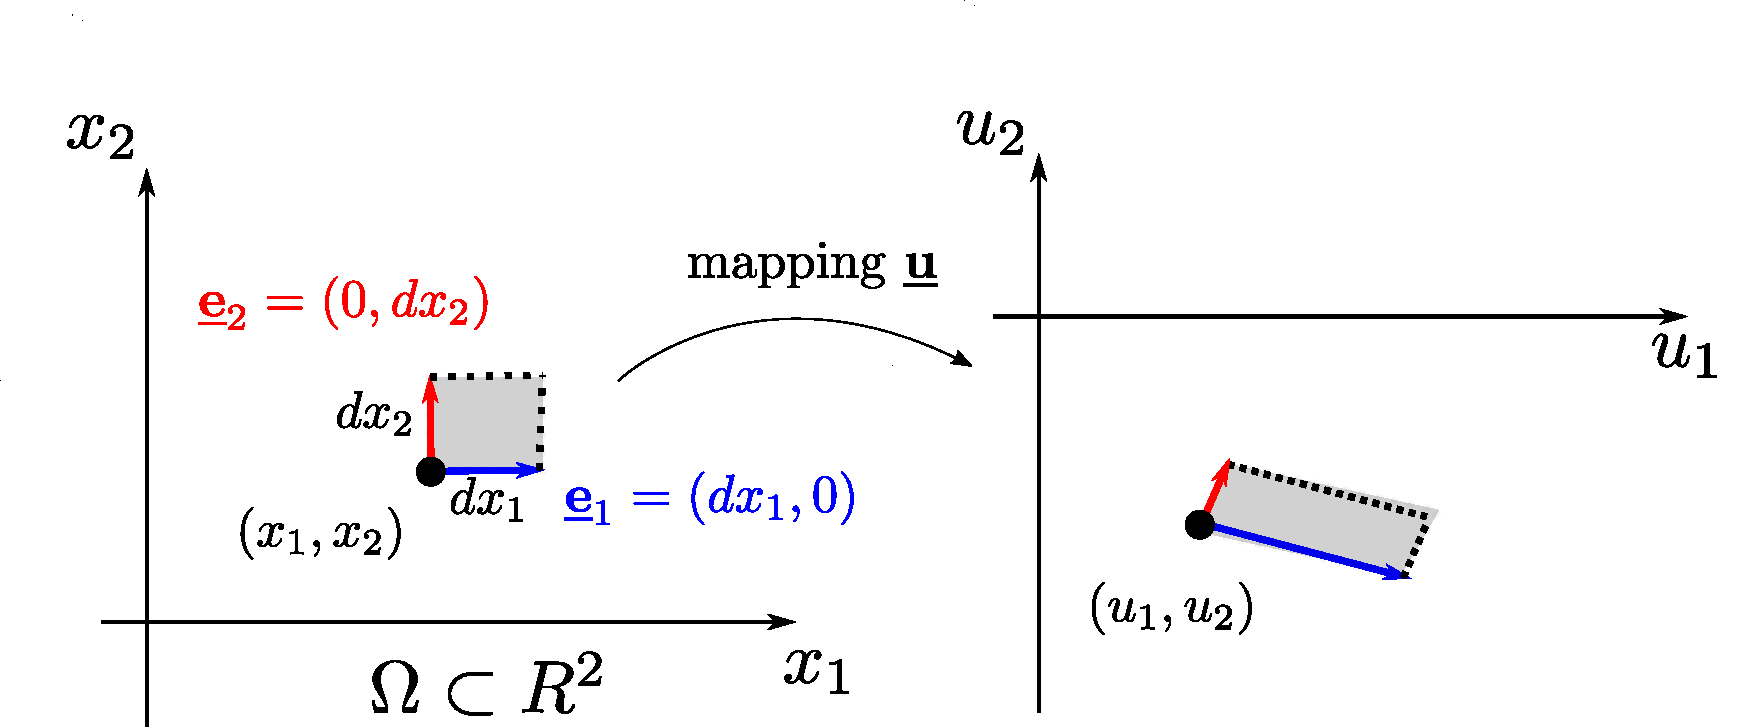
\includegraphics[width=0.7\textwidth]{img/u.pdf}
%\caption*{$\vec{\psi} \in \mathcal{F} = \overline{\operatorname{span} \vec{\phi}(\mathbb{R}^N)}$}
%\end{figure}

The area of the small rectangle in $\Omega$ is $A = dx_1\, dx_2$.\\

The goal is to show that in order for probability to be conserved, the areas on both spaces have to be equal. 
We will therefore demonstrate that:
$$
\int_{\Omega} f(\vec{x}) \mathbf{d}\vec{x}
=\int_{u(\Omega)} f({\vec x(\vec u)}) \frac{1}{\left|\det \frac{\partial \vec{u}(\vec{x})}{\partial \vec{x}} \right|} \mathbf{d}\vec{u}.
$$

\begin{itemize}
\item Because $dx_1$ and $dx_2$ are \emph{infinitesimally small} we can consider the mapping 
$\vec u$ to act as a linear transformation, resulting in a different shape in $u(\Omega)$. 
\item The shape of the shaded area in $u(\Omega)$ is \emph{approximately} a parallelogram.
\item We will compute the ratio of the areas between the two transforms.
\item If we want to go back from $u(\Omega)$ to $\Omega$ we only need $\frac{1}{\text{ratio}}$.
\end{itemize}

\underline{Important:}
Approximating the above as a linear transformation (i.e. a small rectangle turns into a parallelogram) only holds because for very small $d\vec x$.

To get the area of the parallelogram in $u(\Omega)$ we need to find out what $\vec u(dx_1, dx_2))$ is.
The area of the parallelogram then becomes the magnitude of the cross product between the components of $\vec u(\vec x)$.

\newpage

We first only consider the vector due to $dx_1$ in blue:

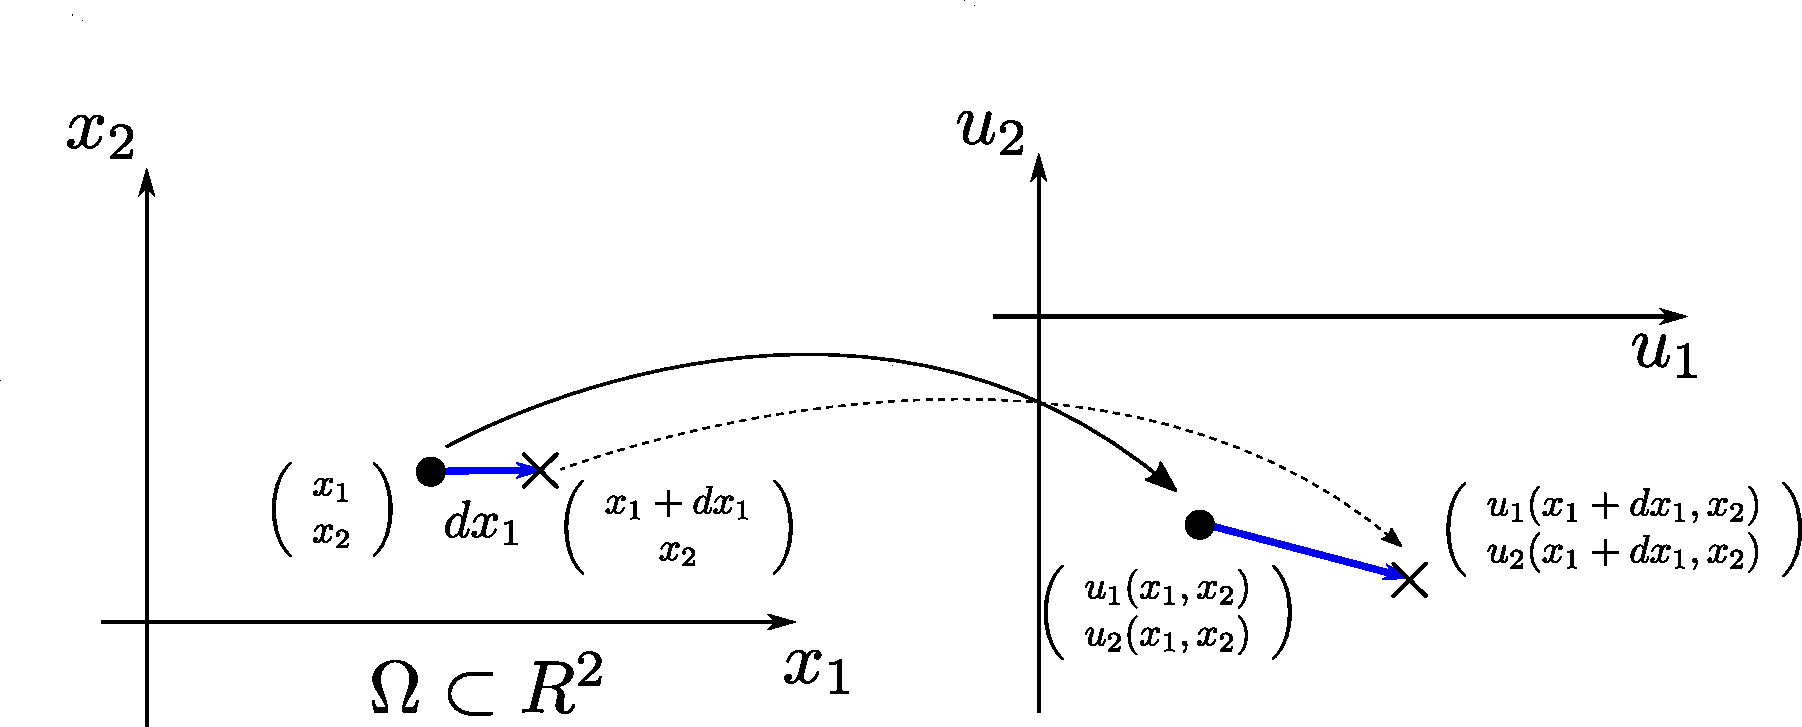
\includegraphics[width=0.75\textwidth]{img/x1.pdf}

The difference vector between the two correspsonding points in $u(\Omega)$ becomes:

\begin{equation*}
\begin{array}{r}
\rmat{
u_1 (x_1 + dx_1, x_2)\\
u_2 (x_1 + dx_2, x_2)
} - 
\rmat{
u_1 (x_1, x_2)\\
u_2 (x_1, x_2)
} \\[0.7cm]
=
\rmat{
u_1 (x_1 + dx_1, x_2) - u_1 (x_1, x_2)\\
u_2 (x_1 + dx_2, x_2) - u_2 (x_1, x_2)
}
\end{array}
\end{equation*}

Because $dx_1$ is so small, we can approximate the transformed vector by the derivative, 
which is essentially taking the limit. The difference vector in $u(\Omega)$ becomes:

$$
u: \vec e_1 \mapsto 
\rmat{
\frac{\partial u_1}{\partial x_1} \Delta x_1\\[0.2cm]
\frac{\partial u_2}{\partial x_1} \Delta x_1
}
$$

\question{What about $dx_2$?}

- We use the same procedure (one the red vector $\vec e_2$) and get:

$$
u: \vec e_2 \mapsto 
\rmat{
\frac{\partial u_1}{\partial x_2} \Delta x_2\\[0.2cm]
\frac{\partial u_2}{\partial x_2} \Delta x_2
}
$$

The area of the parallelogram spanned by the two difference vectors in $u(\Omega)$ 
is the magnitude of their cross product:
\begin{align*}
&\left| \; 
\rmat{
\frac{\partial u_1}{\partial x_1} \Delta x_1\\[0.2cm]
\frac{\partial u_2}{\partial x_1} \Delta x_1
}
\times
\rmat{
\frac{\partial u_1}{\partial x_2} \Delta x_2\\[0.2cm]
\frac{\partial u_2}{\partial x_2} \Delta x_2
}
\; \right|\\ 
&=
\left| \; 
\underbrace{
\frac{\partial u_1}{\partial x_1} \frac{\partial u_2}{\partial x_2}
\; - \;
\frac{\partial u_1}{\partial x_2} \frac{\partial u_2}{\partial x_1}
}_{\text{the Jacobian determinant}}
\; \right| \Delta x_1 \Delta x_2 \\
&= 
\left| \; \det \quad
\underbrace{
\left(
\frac{\partial (u_1, u_2)}{\partial (x_1,x_2)}
\right)
}_{\text{the Jacobian}}
\; \right| \Delta x_1 \Delta x_2
\end{align*}

This matrix of partial derivatives is called the \emph{Jacobian}:
$$
\frac{\partial (u_1, u_2)}{\partial (x_1,x_2)} = 
\frac{\partial (u_1(\vec x), u_2(\vec x))}{\partial (x_1,x_2)} = 
\frac{\partial (\vec u(\vec x))}{\partial (\vec x)} =
\underbrace{
\rmat{
{\partial u_1}/{\partial x_1} & {\partial u_1}/{\partial x_2}\\[0.2cm]
{\partial u_2}/{\partial x_1} & {\partial u_2}/{\partial x_2}
}%rmat
}_{
\substack{
\text{matrix of}\\
\text{partial derivatives}
}%substack
}
$$

If we are given an area spanned by too small vectors (e.g. $\vec e_1$, $\vec e_2$) 
we can compute the area of the corresponding parallelogram in $u(\Omega)$ 
by multiplying the original area by the Jacobian determinant.

\question{What if we want to transform from $u(\Omega)$ back to $\Omega$?}

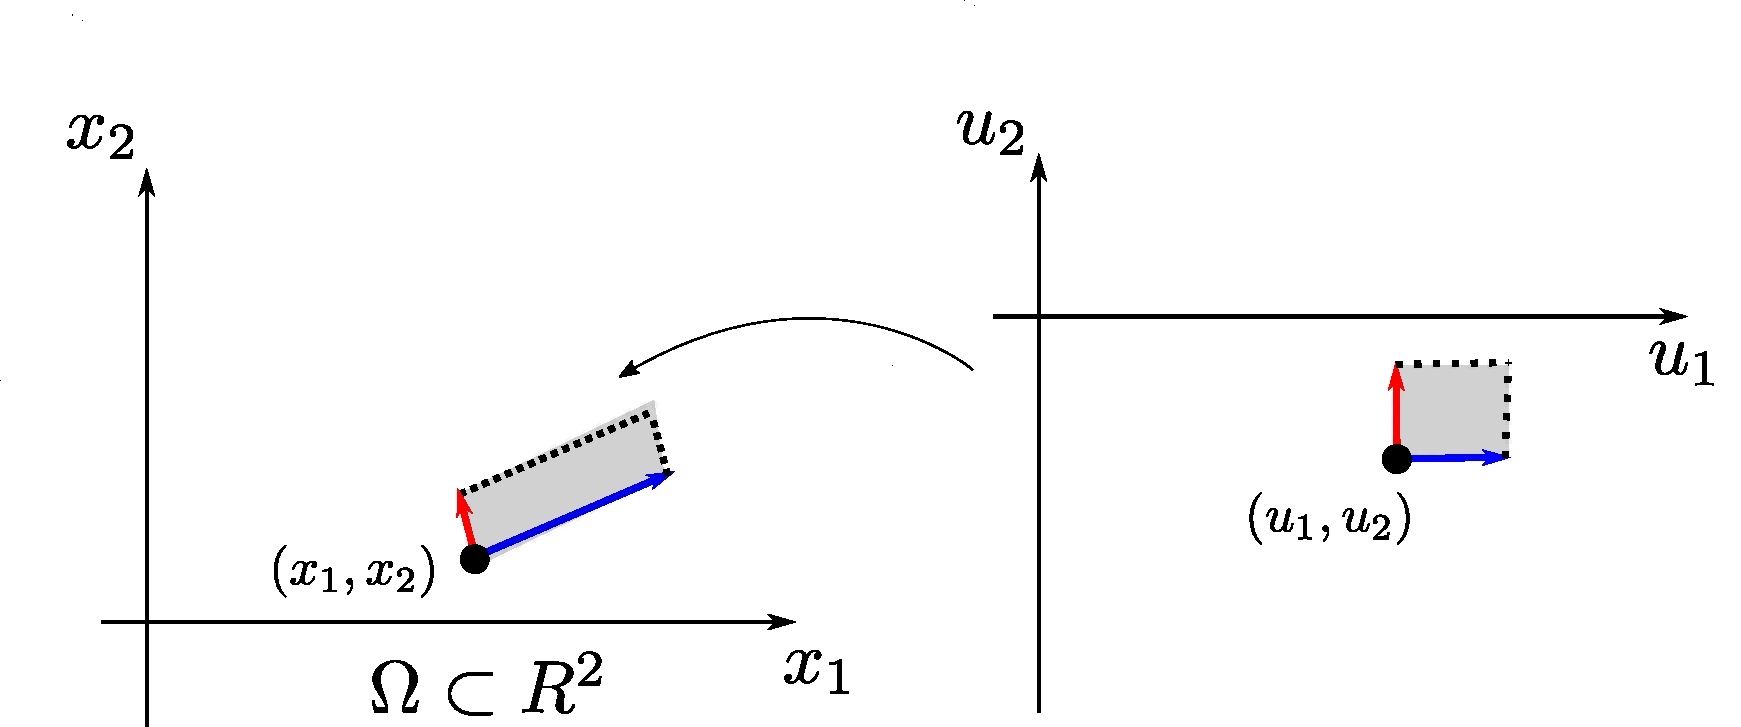
\includegraphics[width=0.7\textwidth]{img/reverse.pdf}

We apply the inverse mapping. A very small rectangle in $u(\Omega)$ transforms into a parallelogram in $\Omega$. 
This reverse transformation would require the inverse of the above matrix of partial derivatives.
The matrix of partial derivatives tells us how to transform infinitesimally small vectors back and forth.

%Transformation between the spaces for infinitesimally small vectors:

%$$
%\rmat{
%u_1(x_1) & u_1(x_2)\\
%u_2(x_1) & u_2(x_2)
%}
%\rmat{
%a\\
%b
%}
%=
%\rmat{
%u_1(x_1)\\
%u_2(x_1)
%}
%a
%+
%\rmat{
%u_1(x_2)\\
%u_2(x_2)
%}
%b
%$$

\question{Do we really have to compute the inverse of the matrix?}

- No, the determinant of the inverse matrix is 1 / det of the original matrix:
$$
\frac{1}{\left| \det \left( \frac{\partial \vec u}{\partial \vec x} \right) \right|} =
{\left| \det \left( \frac{\partial \vec x}{\partial \vec u} \right) \right|}
$$

\underline{Transformation between probability densities:}

Conservation of probability: The area represents the probability of the event, 
transforming it into another space should nt cause any increase or decrease in the probability of the event.

Therefore, if we multiply the area of the rectangle in $\Omega$ by the pdf $f(\vec x)$ at $\vec x$, we get the probability of the parallelogram in $u(\Omega)$:

$$
\int_{\Omega} f(\vec{x}) \mathbf{d}\vec{x}
=\int_{u(\Omega)} f({\vec x(\vec u)}) \left|\det \frac{\partial \vec{x}(\vec{u})}{\partial \vec{u}} \right| \mathbf{d}\vec{u}
$$
$$
=\int_{u(\Omega)} f({\vec x(\vec u)}) \frac{1}{\left|\det \frac{\partial \vec{u}(\vec{x})}{\partial \vec{x}} \right|} \mathbf{d}\vec{u}.
$$

